% Springer classic template (svjour3)
\documentclass{svjour3}

\usepackage[utf8]{inputenc}
\usepackage[T1]{fontenc}
\usepackage{lmodern}
\usepackage{fix-cm}
\renewcommand{\rmdefault}{lmr}
\renewcommand{\sfdefault}{lmss}
\renewcommand{\ttdefault}{lmtt}
\usepackage{microtype}
\usepackage{silence}
\WarningFilter{latex}{Command \showhyphens has changed.}
\usepackage{amsmath,amssymb,mathtools}
\usepackage{booktabs}
\usepackage{array}
\usepackage{enumitem}
\usepackage{graphicx}
\usepackage{tikz}
\usetikzlibrary{arrows.meta,positioning,calc,shapes.geometric}
\usepackage{natbib}
\setcitestyle{authoryear,round}
\usepackage{xurl}
\usepackage[hidelinks]{hyperref}
\usepackage{orcidlink}

\title{Hollow Purple Semantic Nullification: Contradiction-Induced Instability in Language-Model Representation Space}
\titlerunning{Semantic Nullification in Contradictory Prompts}

\author{Aryan Singh Chandel\,\orcidlink{0009-0007-1774-2480}}
\authorrunning{A. S. Chandel}

\institute{Aryan Singh Chandel \at
  RJIT (Rustamji Institute of Technology), Gwalior, India \\
  \email{aryansingh19gh@gmail.com}
}

\journalname{Preprint}
\date{June 26, 2026}

\makeatletter
\@ifundefined{definition}{\spnewtheorem{definition}{Definition}{\bfseries}{\rmfamily}}{}
\@ifundefined{assumption}{\spnewtheorem{assumption}{Assumption}{\bfseries}{\rmfamily}}{}
\@ifundefined{proposition}{\spnewtheorem{proposition}{Proposition}{\bfseries}{\itshape}}{}
\makeatother
\raggedbottom
\emergencystretch=3em

\begin{document}
\maketitle

\begin{abstract}
Contradiction in language models is usually treated as a labeling problem, not as a question about contextual stability. We ask whether prompts that force incompatible commitments into a single local context produce a measurable instability regime beyond ordinary prompt difficulty. To make that question testable, we define a semantic nullification index that aggregates predictive entropy, representation drift, and output inconsistency under matched controls. We then specify a benchmark with explicit control conditions, estimands, decision rules, and falsifiers, and run a seed experiment on three public SNLI-derived contradiction families. The initial evidence is mixed: the measurement pipeline is executable and informative, but the present seed run does not support a clean contradiction threshold. That result sharpens the theory by ruling out weaker, more rhetorical versions of the claim.
\keywords{Language models \and Contradiction \and Semantic instability \and Benchmarking \and Representation analysis}
\end{abstract}

\section{Introduction}
Distributional semantics has long shown that lexical opposition and lexical similarity do not separate neatly in ordinary vector spaces. Words that are conceptually opposed often remain geometrically close because they appear in similar discourse environments \citep{hill2015simlex,mrksic2016counterfitting}. Transformer language models complicate the picture further: meaning is not read off a single embedding, but assembled through repeated contextual mixing across layers and positions \citep{vaswani2017attention}. If contradiction-sensitive failure exists, it is therefore more plausible as a dynamical instability pattern than as a simple antonym direction in representation space.

The question in this paper is narrower than generic ``reasoning failure.'' We ask whether contradiction-rich prompts induce a distinct instability regime after controlling for topic, length, discourse style, and generic semantic density. The motivating metaphor is vivid, but the paper does not ask the reader to believe in literal cancellation inside a transformer. Its aim is more disciplined: convert an evocative intuition into explicit observables and then subject that formulation to the possibility of failure.

\paragraph{Contributions.}
\begin{enumerate}[leftmargin=*]
\item We define a semantic nullification index that aggregates predictive entropy, representation drift, and output inconsistency.
\item We specify a contradiction benchmark with coherent controls, difficulty-matched non-contradictory controls, explicit contradictions, and nested contradictions.
\item We give formal hypotheses, test statistics, decision rules, and falsifiers that separate contradiction effects from ordinary prompt difficulty.
\item We report a public-data seed measurement on three SNLI-derived prompt families using a fixed model and fixed decoding protocol.
\end{enumerate}

\section{Formal Setup}
Let $x^{(0)}$ denote a matched control prompt and $x^{(c)}$ a contradiction-bearing prompt. Let $p_\theta(\cdot \mid x_{<t})$ be the next-token distribution at position $t$, and let $h_\ell(x)\in\mathbb{R}^{d_\ell}$ be a layer summary at layer $\ell$.

\begin{definition}[Contradiction depth]
The contradiction depth of prompt $x$ is a normalized score $d(x)\in[0,1]$ that measures the density of mutually incompatible semantic commitments relative to the number of proposition-bearing clauses in $x$.
\end{definition}

\begin{definition}[Entropy response]
For a monitored token set $T(x)$, define the mean predictive entropy
\[
H(x)=\frac{1}{|T(x)|}\sum_{t\in T(x)}\left(-\sum_v p_\theta(v\mid x_{<t})\log p_\theta(v\mid x_{<t})\right).
\]
\end{definition}

\begin{definition}[Representation drift]
For a matched pair $(x^{(c)},x^{(0)})$, the layerwise representation drift is
\[
\Delta_\ell(x^{(c)},x^{(0)})=1-\cos\!\big(h_\ell(x^{(c)}),h_\ell(x^{(0)})\big).
\]
\end{definition}

\begin{definition}[Output inconsistency]
Let $y_s(x)$ be the response under seed $s$ and let $\phi(y_s(x))$ be a fixed response-code mapping (for example, entailment-compatible, contradiction-compatible, or evasive). The output inconsistency score is
\[
I(x)=1-\frac{1}{|S|(|S|-1)}\sum_{s\neq s'} \mathbf{1}\{\phi(y_s(x))=\phi(y_{s'}(x))\}.
\]
\end{definition}

\begin{definition}[Semantic nullification index]
Let $\widetilde{H}(x)$, $\widetilde{\Delta}(x)$, and $\widetilde{I}(x)$ denote standardized forms of entropy, drift, and inconsistency under a declared benchmark. The semantic nullification index is
\[
N(x)=w_H\widetilde{H}(x)+w_\Delta\widetilde{\Delta}(x)+w_I\widetilde{I}(x),
\]
where $w_H,w_\Delta,w_I\ge 0$ and $w_H+w_\Delta+w_I=1$.
\end{definition}

\begin{definition}[Family-level contrast]
For contradiction family $f$ with contradiction-bearing set $\mathcal{X}^{(c)}_f$ and difficulty-control set $\mathcal{X}^{(d)}_f$, define
\[
\delta_f=
\frac{1}{|\mathcal{X}^{(c)}_f|}\sum_{x\in\mathcal{X}^{(c)}_f}N(x)
\;-\;
\frac{1}{|\mathcal{X}^{(d)}_f|}\sum_{x\in\mathcal{X}^{(d)}_f}N(x).
\]
\end{definition}

\begin{definition}[Threshold sensitivity]
For a candidate contradiction threshold $\tau$, define
\[
G(\tau)=
\mathbb{E}[N(x)\mid d(x)\ge \tau]
-
\mathbb{E}[N(x)\mid d(x)<\tau].
\]
The threshold conjecture predicts that $G(\tau)$ becomes positive on a nondegenerate interval rather than only at isolated values of $\tau$.
\end{definition}

\begin{table}[t]
\centering
\small
\caption{Core notation used throughout the manuscript.}
\label{tab:hp-notation}
\begin{tabular}{ll}
\toprule
Symbol & Meaning \\
\midrule
$x$ & prompt instance \\
$d(x)$ & contradiction depth score \\
$H(x)$ & mean predictive entropy \\
$\Delta_\ell(x^{(c)},x^{(0)})$ & layerwise representation drift \\
$I(x)$ & output inconsistency across seeds \\
$N(x)$ & semantic nullification index \\
$T_N$ & primary between-condition contrast \\
$\tau$ & contradiction-depth threshold under the theory \\
\bottomrule
\end{tabular}
\end{table}

\section{Assumptions and Propositions}
\begin{assumption}[Prompt comparability]
Matched prompt families preserve topic, approximate length, discourse mode, and lexical rarity closely enough that contradiction depth is the main manipulated factor.
\end{assumption}

\begin{assumption}[Observable instability]
If contradiction-sensitive instability exists, it leaves a measurable trace in at least one of entropy, representation drift, or output inconsistency.
\end{assumption}

\begin{assumption}[Paraphrase robustness]
A genuine contradiction effect should persist under paraphrase families that preserve incompatibility while varying surface form.
\end{assumption}

\begin{proposition}[Threshold conjecture]
If semantic nullification exists as a contradiction-sensitive regime, then there is a contradiction-depth threshold $\tau$ such that
\[
\mathbb{E}[N(x)\mid d(x)\ge\tau]>\mathbb{E}[N(x)\mid d(x)<\tau].
\]
\end{proposition}

\begin{proposition}[Difficulty separation]
If semantic nullification is specifically contradiction-driven, then contradiction-bearing prompts should satisfy
\[
\mathbb{E}[N(x)\mid x\in\mathcal{C}_{\text{contr}}]>\mathbb{E}[N(x)\mid x\in\mathcal{C}_{\text{diff}}],
\]
where $\mathcal{C}_{\text{diff}}$ is the set of difficulty-matched but jointly satisfiable controls.
\end{proposition}

\begin{proposition}[Paraphrase persistence]
If the effect is semantic rather than lexical, then the sign of the contradiction-minus-control contrast should be preserved across a paraphrase family $\Pi(x)$ with fixed incompatibility structure.
\end{proposition}

\begin{proposition}[Cross-family stability]
If semantic nullification is not a one-template artifact, then the mean family contrast
\[
\bar{\delta}=\frac{1}{|\mathcal{F}|}\sum_{f\in\mathcal{F}}\delta_f
\]
remains positive under leave-one-family-out re-estimation over the benchmark family set $\mathcal{F}$.
\end{proposition}

\subsection*{Null Hypothesis}
After controlling for semantic density, topic, and approximate length, contradiction-bearing prompts do not produce a larger nullification index than non-contradictory difficulty controls.

\subsection*{Effect-Size Target}
For an early-stage benchmark, a practically meaningful signal is a standardized mean difference of at least $0.5$ in $N(x)$ between contradiction-bearing prompts and difficulty-matched controls.

\section{Benchmark Design}
Each prompt family contains four variants: a coherent control, a non-contradictory difficulty control, an explicit contradiction, and a nested contradiction. This structure is deliberately stricter than a simple contradiction-versus-control split because contradiction often co-occurs with increased semantic density.

\begin{table}[t]
\centering
\small
\caption{Condition structure for the semantic nullification benchmark.}
\label{tab:hp-conditions}
\begin{tabular}{p{0.22\linewidth}p{0.18\linewidth}p{0.44\linewidth}}
\toprule
Condition & Target depth & Construction principle \\
\midrule
Control & low & coherent premise-hypothesis realization \\
Difficulty control & low--mid & denser but jointly satisfiable variant \\
Explicit contradiction & mid--high & one direct incompatibility with the premise \\
Nested contradiction & high & multiple cross-clause incompatible commitments \\
\bottomrule
\end{tabular}
\end{table}

\begin{table}[t]
\centering
\small
\caption{Measured variables and their inferential role.}
\label{tab:hp-variables}
\begin{tabular}{p{0.28\linewidth}p{0.18\linewidth}p{0.40\linewidth}}
\toprule
Observable & Symbol & Role in analysis \\
\midrule
Predictive entropy & $H(x)$ & local uncertainty inflation \\
Representation drift & $\Delta_\ell$ & contextual displacement from control \\
Output inconsistency & $I(x)$ & behavioral instability across seeds \\
Nullification index & $N(x)$ & primary aggregate endpoint \\
\bottomrule
\end{tabular}
\end{table}

\section{Identification Strategy}
The identification problem is straightforward to state: contradiction is often confounded with generic difficulty, lexical rarity, or benchmark artifacts. The benchmark addresses this in three ways. First, each contradiction prompt is paired with a coherent control and a difficulty-matched non-contradictory control. Second, contradiction can be realized through lexical, temporal, causal, role-based, or world-knowledge incompatibility rather than through overt negation alone. Third, the benchmark is evaluated at family level so that one striking item cannot dominate interpretation.

\begin{figure}[t]
\centering
\resizebox{\linewidth}{!}{%
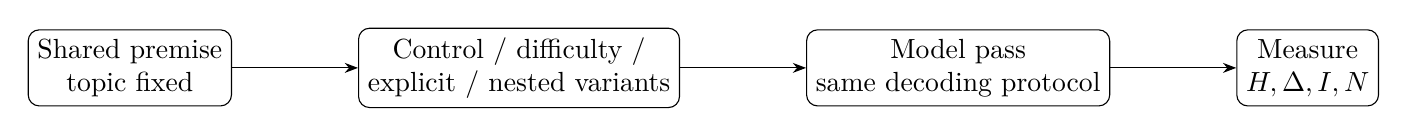
\begin{tikzpicture}[node distance=1.6cm,>=Stealth]
\node[draw,rounded corners,align=center] (a) {Shared premise\\topic fixed};
\node[draw,rounded corners,right=of a,align=center] (b) {Control / difficulty /\\explicit / nested variants};
\node[draw,rounded corners,right=of b,align=center] (c) {Model pass\\same decoding protocol};
\node[draw,rounded corners,right=of c,align=center] (d) {Measure\\$H,\Delta,I,N$};
\draw[->] (a) -- (b);
\draw[->] (b) -- (c);
\draw[->] (c) -- (d);
\end{tikzpicture}
}
\caption{Family construction and measurement pipeline. Contradiction depth, rather than topic, drives the primary contrast.}
\label{fig:hp-flow}
\end{figure}

\begin{figure}[t]
\centering
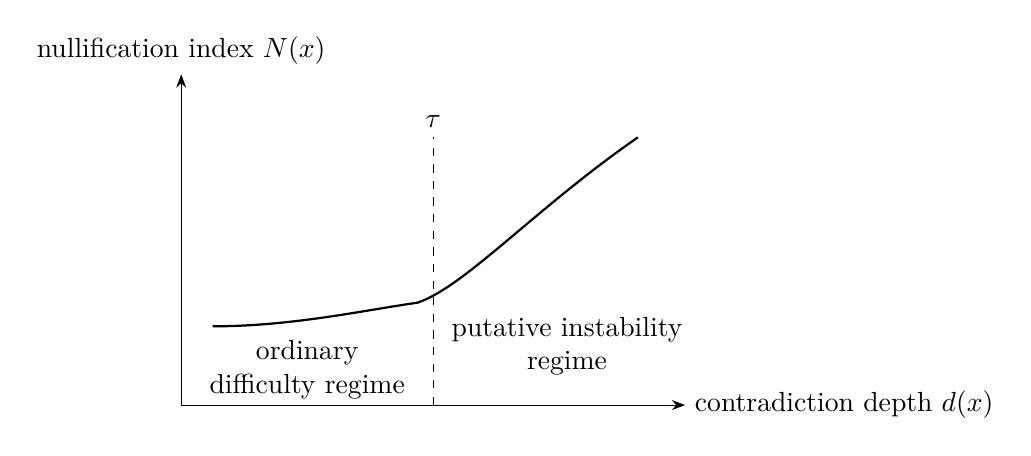
\begin{tikzpicture}[>=Stealth]
\draw[->] (0,0) -- (6.4,0) node[right] {contradiction depth $d(x)$};
\draw[->] (0,0) -- (0,4.2) node[above] {nullification index $N(x)$};
\draw[dashed] (3.2,0) -- (3.2,3.4) node[above] {$\tau$};
\draw[thick] (0.4,1.0) .. controls (1.4,1.0) and (2.3,1.2) .. (3.0,1.3)
             .. controls (3.6,1.5) and (4.5,2.5) .. (5.8,3.4);
\node[align=center] at (1.6,0.45) {ordinary\\difficulty regime};
\node[align=center] at (4.9,0.75) {putative instability\\regime};
\end{tikzpicture}
\caption{Threshold-style interpretation of the theory. The figure is conceptual rather than empirical: the seed experiment is explicitly allowed to reject this pattern.}
\label{fig:hp-threshold}
\end{figure}

\begin{figure}[t]
\centering
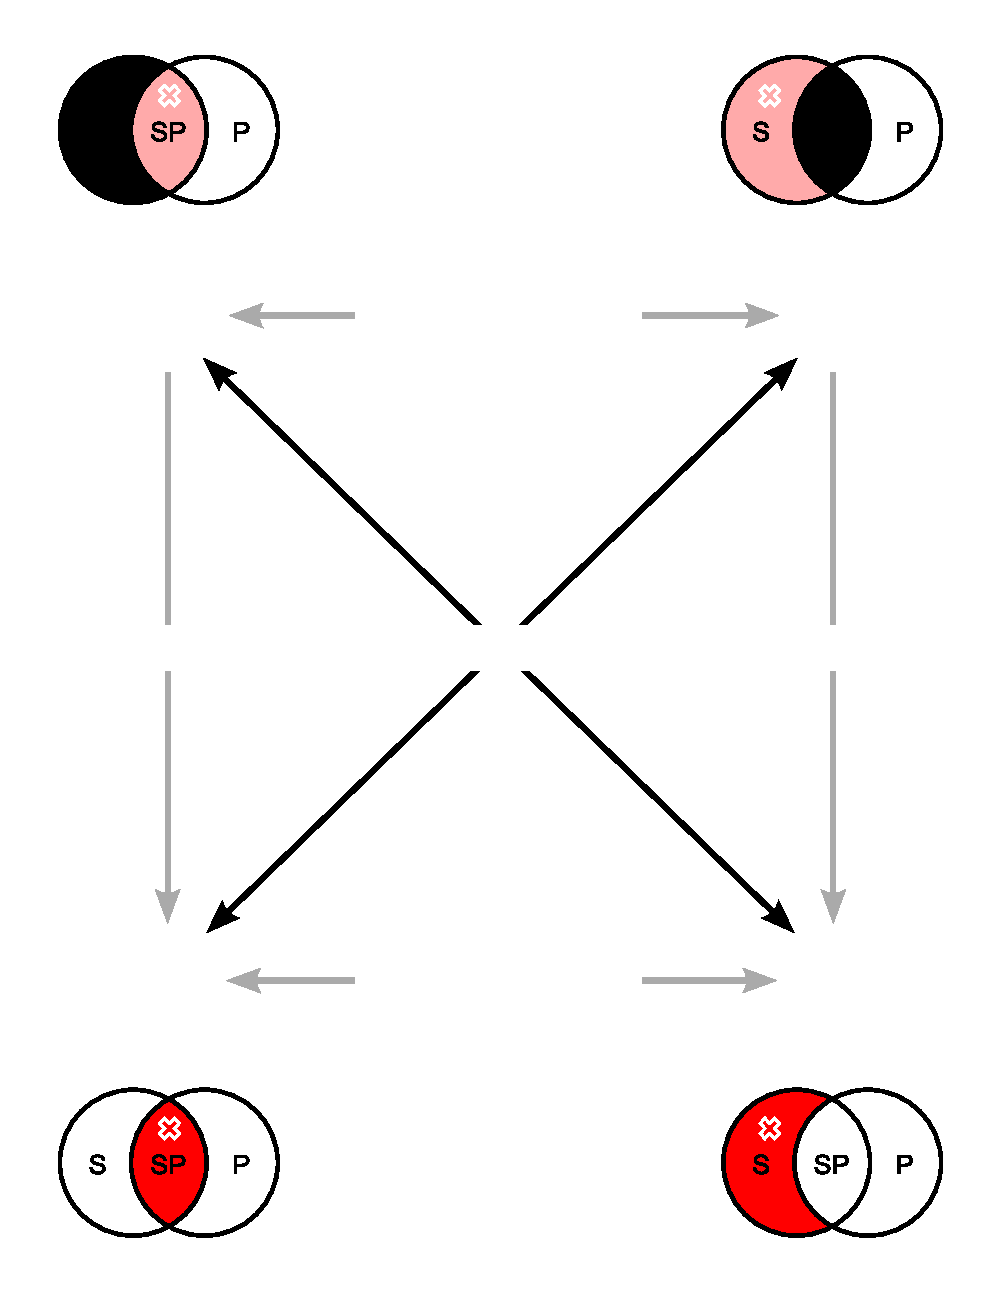
\includegraphics[width=0.62\linewidth]{figures/square_of_opposition_set_diagrams.pdf}
\caption{Classical opposition structure provides a useful logical baseline for contradiction-sensitive prompt construction. Included from a public-domain Wikimedia Commons figure \citep{wikimedia_square_opposition}.}
\label{fig:hp-square}
\end{figure}

\section{Methodology}
\subsection{Model and Public Data}
The seed benchmark is populated from public SNLI-derived contradiction families \citep{bowman2015snli}. The current seed run uses \texttt{distilgpt2} under fixed decoding settings so that observed variation is attributable to prompt family differences rather than to policy drift during sampling.

\subsection{Primary Test Statistic}
Let $\mathcal{X}_{\text{contr}}$ denote contradiction-bearing prompts and $\mathcal{X}_{\text{ctrl}}$ the matched coherent controls. The primary contrast is
\[
T_N=\overline{N}_{\text{contr}}-\overline{N}_{\text{ctrl}}.
\]
For the sharper test against generic difficulty, define
\[
T_N^{\star}=\overline{N}_{\text{contr}}-\overline{N}_{\text{diff}},
\]
where $\overline{N}_{\text{diff}}$ is the mean nullification index under difficulty-matched non-contradictory controls.

Because a single family can be unusually noisy, we also estimate the family-aggregated contrast
\[
\widehat{\bar{\delta}}=\frac{1}{|\mathcal{F}|}\sum_{f\in\mathcal{F}}\widehat{\delta}_f
\]
and treat sign stability of $\widehat{\delta}_f$ across families as part of the inferential target rather than a secondary diagnostic.

\subsection{Estimator and Uncertainty}
Let $B$ denote the number of bootstrap resamples drawn at family level. The reported uncertainty interval for $T_N^{\star}$ is
\[
\left[\widehat{T}_{N,(0.025)}^{\star},\widehat{T}_{N,(0.975)}^{\star}\right],
\]
where the quantiles are taken over bootstrap replicates that resample prompt families, not individual generations. This choice aligns the uncertainty estimate with the unit of scientific generalization.

\subsection{Standardized Effect Size}
To complement raw contrasts, we recommend the family-pooled standardized effect
\[
g_N=\frac{\overline{N}_{\text{contr}}-\overline{N}_{\text{diff}}}
{\sqrt{\tfrac{1}{2}\left(\widehat{\sigma}_{\text{contr}}^2+\widehat{\sigma}_{\text{diff}}^2\right)}}.
\]
This prevents small but noisy raw differences from being mistaken for substantive contradiction effects.

\subsection{Regression-Form Identification}
To separate contradiction effects from correlated prompt properties, we recommend the family-fixed-effects model
\[
N(x)=\alpha_{f(x)}+\beta_d d(x)+\beta_\ell L(x)+\beta_r R(x)+\beta_q Q(x)+\varepsilon_x,
\]
where $\alpha_{f(x)}$ is a family intercept, $L(x)$ is normalized length, $R(x)$ is lexical rarity, and $Q(x)$ is semantic-density or proposition-count proxy. Under the theory, $\beta_d>0$ should persist after adjustment.

\subsection{Randomization Test}
Because benchmark families are small, a finite-sample alternative to asymptotic inference is a within-family label permutation test. Let $\pi_f$ range over condition-label permutations preserving family structure. The exact or Monte Carlo $p$-value is
\[
p_{\mathrm{perm}}=\Pr_{\pi}\!\left(\widehat{T}_{N,\pi}^{\star}\ge \widehat{T}_{N}^{\star}\right).
\]
This test is valid under exchangeability of contradiction and difficulty labels within matched families.

\subsection{Decision Rule}
The theory is treated as provisionally supported only if three conditions hold jointly:
\begin{enumerate}[leftmargin=*]
\item $T_N^{\star}>0$ with a pre-registered confidence interval excluding zero;
\item the sign of the contrast is stable across contradiction families rather than driven by one outlier;
\item the effect persists under paraphrase-preserving variants.
\end{enumerate}

For a more stringent benchmark, all three conditions should hold together with $\widehat{\beta}_d>0$ in the regression specification and $p_{\mathrm{perm}}<0.05$ under family-preserving permutations.

\subsection{Control Condition}
The control condition preserves topic, discourse form, and approximate proposition count while removing incompatible commitments. The difficulty control preserves density and elaboration while keeping the prompt jointly satisfiable.

\subsection{Confound Checklist}
\begin{itemize}[leftmargin=*]
\item overt negation markers that act as superficial cues,
\item lexical rarity raising entropy without contradiction,
\item prompt-length differences altering attention allocation,
\item annotation artifacts that leak the contradiction label,
\item response-scoring schemes that confuse uncertainty with inconsistency.
\end{itemize}

\subsection{What Counts as Evidence}
This theory is empirical rather than deductive. Evidence in favor of semantic nullification requires replicated between-condition contrasts, stability across paraphrase families, and separation from difficulty controls. A formal proof is available only for the benchmark definitions or estimator properties, not for the existence of the phenomenon itself.

More specifically, we treat the theory as strengthened when four items align: positive $T_N^{\star}$, positive $\widehat{\bar{\delta}}$, no single family dominating the sign of the aggregate effect, and no alternative observable such as lexical rarity explaining the contrast better in matched regression checks.

\subsection{What Falsifies the Theory}
The theory weakens materially if contradiction fails to exceed difficulty controls, if drift is explained better by lexical rarity than by incompatibility, or if the effect vanishes once paraphrase and negation cues are balanced. These are not peripheral caveats; they are the main exit routes from the hypothesis.

An especially strong falsifier is sign reversal after covariate control: if $\widehat{\beta}_d\le 0$ in the adjusted model across multiple model families, then the contradiction-depth variable is not isolating a distinct instability process.

\section{Seed Measurement}
\subsection{Public-Data Run}
We executed the seed benchmark on three public contradiction families using \texttt{distilgpt2}. The purpose of this pass was not to claim discovery of a new regime, but to verify that the benchmark and scoring pipeline produce interpretable values on real data.

\begin{table}[t]
\centering
\small
\caption{Seed-scale nullification indices measured on three public contradiction families.}
\label{tab:hp-seed}
\begin{tabular}{lcccc}
\toprule
Family & Control & Difficulty & Explicit & Nested \\
\midrule
\texttt{hp\_seed\_001} & 0.1353 & 0.1382 & 0.1324 & 0.1237 \\
\texttt{hp\_seed\_002} & 0.1403 & 0.1424 & 0.1432 & 0.1406 \\
\texttt{hp\_seed\_003} & 0.1323 & 0.1327 & 0.1330 & 0.1274 \\
\bottomrule
\end{tabular}
\end{table}

\begin{table}[t]
\centering
\small
\caption{Condition-wise means across the three seed families.}
\label{tab:hp-mean}
\begin{tabular}{lc}
\toprule
Condition & Mean nullification index \\
\midrule
Control & 0.1360 \\
Difficulty control & 0.1378 \\
Explicit contradiction & 0.1362 \\
Nested contradiction & 0.1306 \\
\bottomrule
\end{tabular}
\end{table}

\begin{figure}[t]
\centering
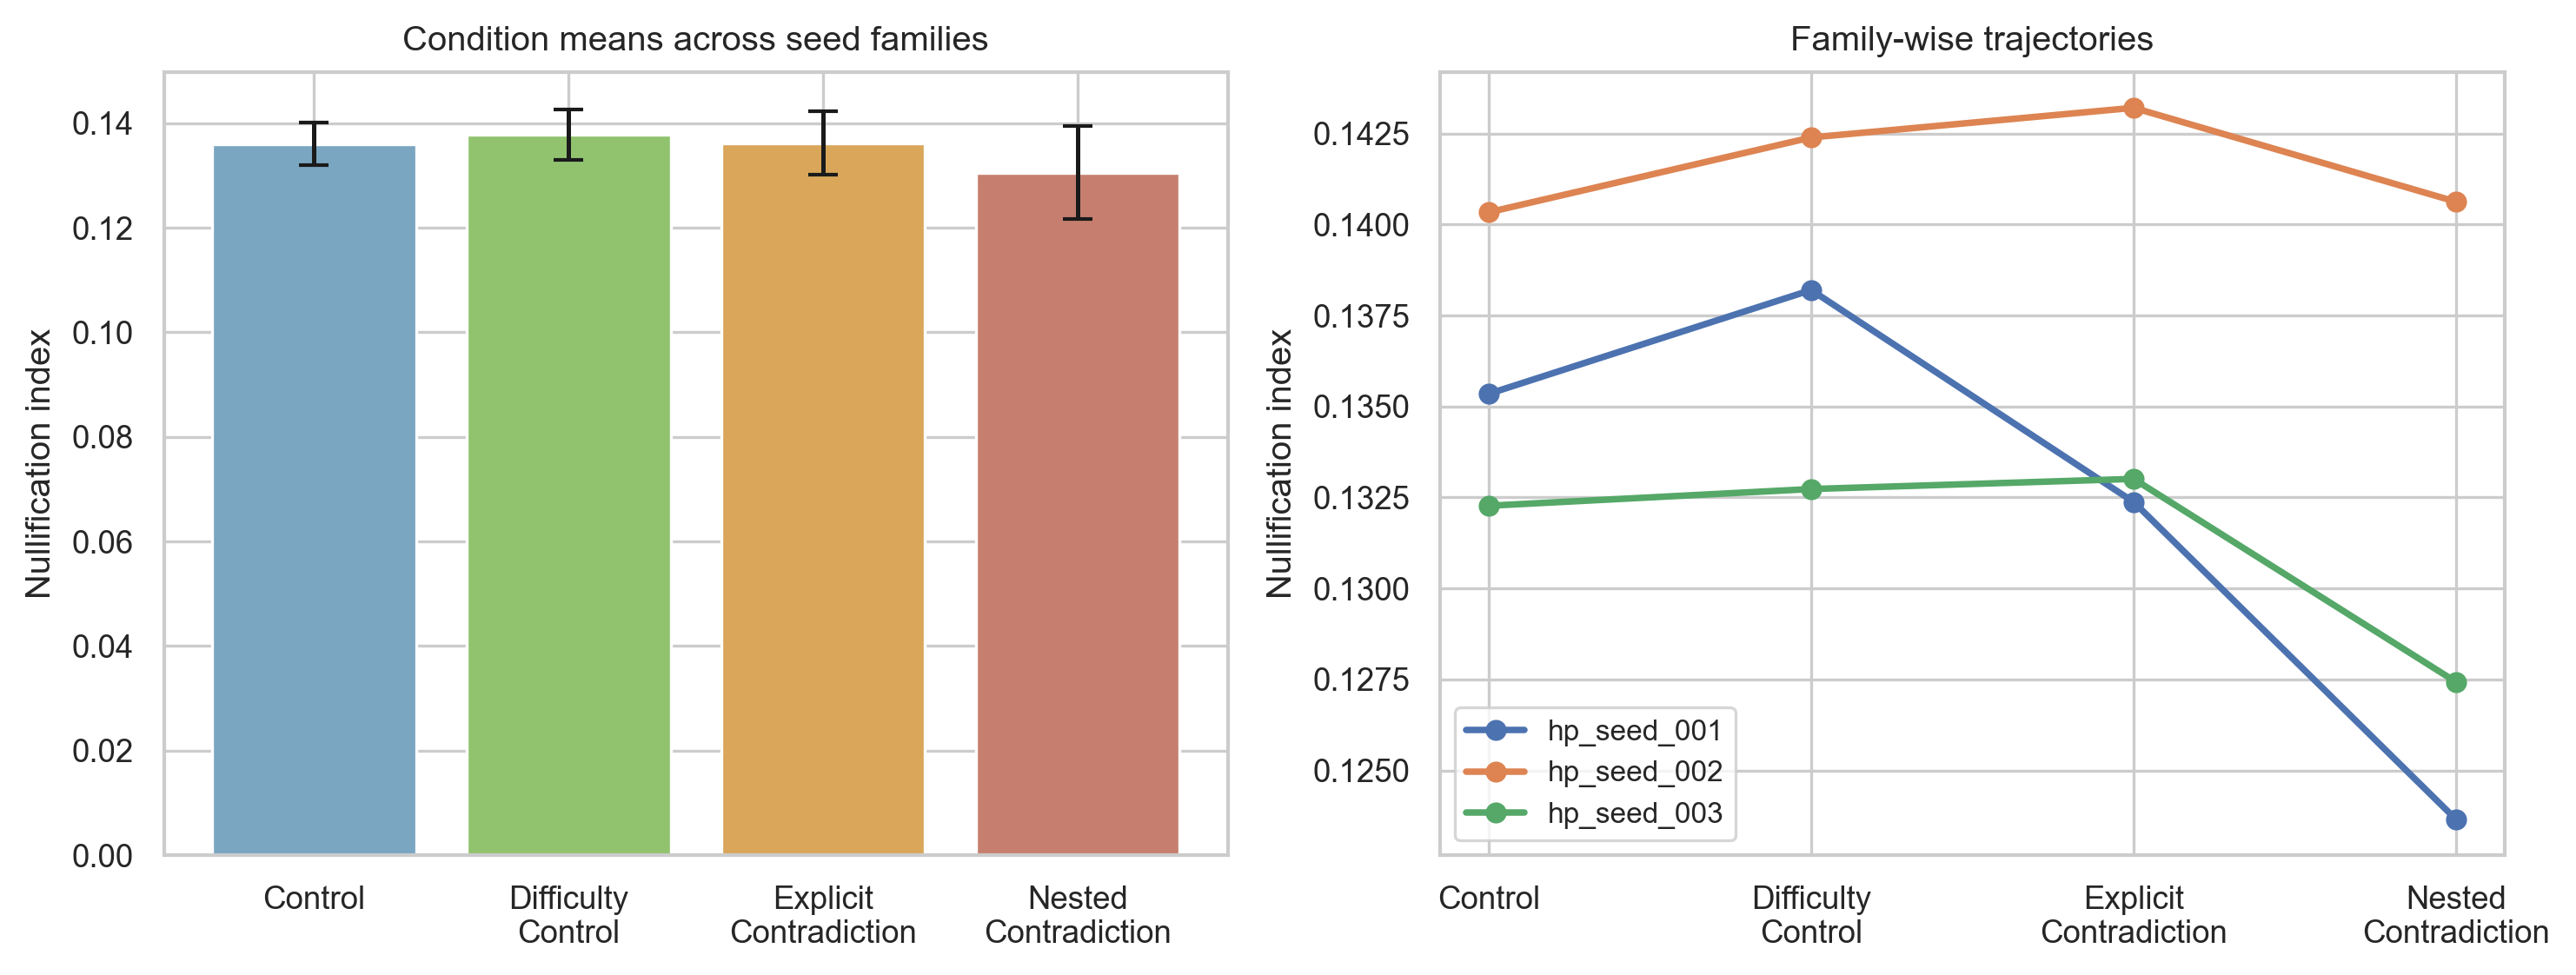
\includegraphics[width=\linewidth]{figures/hollow_purple_seed_results.png}
\caption{Measured seed-scale behavior. Left: condition means with standard-deviation bars across families. Right: family-wise nullification trajectories.}
\label{fig:hp-seed}
\end{figure}

\subsection{Interpretation}
The present seed run does not support a strong threshold claim. One family shows a slight increase from the difficulty control to the explicit contradiction condition, while the aggregate mean does not. Nested contradiction is actually lower on average in this first pass. That result matters. It suggests either that the current nullification index does not yet isolate the proposed mechanism, or that contradiction in this benchmark perturbs generation in a way that is not well captured by the current weights and observables.

Put differently, the seed experiment behaves as a sanity check, not as a victory lap. The pipeline can be run, public data can populate it, and the theory can be disappointed on first contact with measurement. That is exactly the kind of friction a usable theory should permit.

\section{Discussion}
Two points deserve emphasis. First, the benchmark is already informative even without a positive result. A negative or ambiguous seed outcome is still scientifically useful if it narrows the space of plausible claims and identifies where the measurement model is too coarse. Second, the central object of interest may not be contradiction alone, but contradiction under particular representational bottlenecks---for example, when incompatibility is distributed across clauses, roles, or temporal updates in a way that forces deeper integration.

The present evidence therefore supports a restrained conclusion. It is reasonable to keep the semantic nullification hypothesis alive, but only in a sharpened form that makes room for null results, model dependence, and metric misspecification. A publication-worthy version of this project will likely depend less on rhetorical novelty and more on whether contradiction-sensitive effects survive against strong difficulty controls and paraphrase-balanced prompt families.

A useful consequence of the current null result is conceptual hygiene. It discourages treating contradiction as an intrinsically catastrophic signal and instead pushes the theory toward conditional claims about when incompatible commitments become measurably destabilizing. In that sense, the benchmark is already doing what a good theoretical instrument should do: it constrains the story, not just decorates it.

\section{Related Work}
This study sits between vector semantics, contradiction benchmarks, and representation analysis. SimLex and counter-fitting work show why lexical opposition should not be treated as a one-dimensional geometric primitive \citep{hill2015simlex,mrksic2016counterfitting}. SNLI and ANLI provide large-scale contradiction supervision, though primarily as a classification problem \citep{bowman2015snli,nie2019anli}. The literature on NLI artifacts reminds us that contradiction benchmarks can overstate semantic competence when cues are superficial \citep{gururangan2018artifacts}. Finally, recent work at the border of neural and symbolic contradiction analysis reinforces the need to treat contradiction as a structured relation rather than as mere lexical mismatch \citep{feng2024neurosymbolic}.

\section{Limitations and Future Work}
The paper has four immediate limitations. First, the seed benchmark is too small for strong statistical inference. Second, the present run uses one model and one decoding configuration, so it cannot distinguish model-specific quirks from general behavior. Third, the nullification index remains a designed aggregate rather than a validated latent construct. Fourth, the current benchmark still leans on contradiction families that originate in NLI-style data, which may import annotation regularities not present in open-ended prompting.

The most direct next steps are clear: enlarge the public prompt pool, build paraphrase-balanced contradiction families, examine layer-specific drift instead of a single summary, and replicate the analysis across models with fixed reporting standards. Stronger versions of the study should also compare alternative index constructions, report annotation agreement for contradiction depth, and test whether intervention on specific clauses changes instability in predictable ways. If the effect persists under those stronger conditions, the theory becomes materially more credible. If it does not, the framework still succeeds by showing where the metaphor stops being technically useful.

\section{Conclusion}
The phrase \emph{semantic nullification} should stand or fall on measurable behavior. The current benchmark does not yet confirm a contradiction threshold, but it does provide a disciplined way to test one. That is enough reason to keep the theory alive and enough pressure to keep it honest.

\section*{Declarations}
\paragraph{Funding} No external funding was received for this work.
\paragraph{Competing interests} The author declares no competing interests.
\paragraph{Data and materials availability} The benchmark families are derived from publicly available datasets and are available from the corresponding author upon reasonable request.
\paragraph{Code availability} The analysis code used for measurement is available from the corresponding author upon reasonable request.
\paragraph{Author contributions} Aryan Singh Chandel: conceptualization, methodology, formalization, analysis, writing---original draft, writing---review and editing.

\bibliographystyle{spbasic}
\bibliography{references}
\end{document}
